\PassOptionsToPackage{table}{xcolor}
\documentclass[10pt]{beamer}
\usepackage[english]{babel}

\usetheme{metropolis}
\usepackage{smartdiagram}
\usepackage{listings}
\usepackage{booktabs}
\usepackage[scale=2]{ccicons}%creative commons
\setbeamercovered{transparent}%invisible by default
\usepackage{array}
\newcolumntype{L}[1]{>{\raggedright\let\newline\\\arraybackslash\hspace{0pt}}m{#1}}
\newcolumntype{C}[1]{>{\centering\let\newline\\\arraybackslash\hspace{0pt}}m{#1}}
\newcolumntype{R}[1]{>{\raggedleft\let\newline\\\arraybackslash\hspace{0pt}}m{#1}}

\usepackage{pgfplots}
\usepgfplotslibrary{dateplot}
\usepackage{tikz}
\usetikzlibrary{positioning,chains,fit,shapes,calc,automata,positioning}
\newcommand{\mycomment}[1]{}
\usepackage{fancyvrb}
\usepackage{ifpdf}                        % To check if pdflatex is used.

\ifpdf
  \DeclareGraphicsRule{*}{mps}{*}{}       % To include metapost files.
\fi
% *****************************************************************************
% Matematica 
% *****************************************************************************

%\usepackage{amssymb}
%\usepackage{mathtools}                    % Add support for cramped,
					  
%\usepackage[euler]{flexisym}
%\usepackage{breqn}                        % Breqn
%\makeatletter
%   \def\eqnumsize{\normalfont \Tf@font}      % Add support to Minion Pro
%\makeatother
%\setkeys{breqn}{labelprefix={eq:}}


%\usepackage{asymptote}
%\usepackage[loop, controls]{animate}

\graphicspath{{./}, {./Images/}}

\lstdefinelanguage{Kotlin}{
  keywords={package, as, typealias, this, super, val, var, fun, for, null, true, false, is, in, throw, return, break, continue, object, if, try, else, while, do, when, yield, typeof, yield, typeof, class, interface, enum, object, override, public, private, get, set, import, abstract, },
  keywordstyle=\color{blue}\bfseries,
  ndkeywords={@Deprecated, Int, Integer, Float, Double, String, Runnable, dynamic},
  ndkeywordstyle=\color{red}\bfseries,
  emph={println, return@, forEach,},
  emphstyle={\color{red}},
  identifierstyle=\color{black},
  sensitive=true,
  commentstyle=\color{gray}\ttfamily,
  comment=[l]{//},
  morecomment=[s]{/*}{*/},
  stringstyle=\color{gray}\ttfamily,
  morestring=[b]",
  morestring=[s]{"""*}{*"""},
}

\providecommand{\ie}{i.\,e.}
\providecommand{\Ie}{I.\,e.}
\providecommand{\eg}{e.\,g.}
\providecommand{\Eg}{E.\,g.} 

\metroset{block=fill}
\metroset{titleformat frame=smallcaps}

\title{Scala cruise} 
\subtitle{Snorkelling in some of the Scala features}
% crash course in Scala
\date{\today}
\author[A. Candolini]{Alessandro Candolini}
%\institute{Department of Physics, University of Trieste}
% \titlegraphic{\hfill\includegraphics[height=1.5cm]{logo/logo}}

\begin{document}

\maketitle

\begin{frame}{Itinerary}
  \setbeamertemplate{section in toc}[sections numbered]
  \tableofcontents[hideallsubsections]
\end{frame}

\section{Let's meet Scala}

\begin{frame}
\begin{figure}
\centering
\includegraphics[width=.5\textheight]{martin}
\caption{Martin Odersky, the creator of Scala}
\end{figure}
\end{frame}

% Odersky viewpoint influences the look and feel and development of the Scala lang => synergy between OOP and FP 

\begin{frame}[fragile]
Scala programming language is:
\begin{itemize}
\item general purpose 
\item strongly statically typed (with type inference) 
\item compiling primarily to JVM 8+ bytecode%
\footnote{\texttt{scala.js} compiles to JS; \texttt{scala native} targets LLVM; jdk 9+ compatibility might require support; there is a Scala REPL.}
\item interoperable with Java 8+
\end{itemize}
\end{frame}

\begin{frame}
Scala supports 
\begin{itemize}
\item OOP
\item FP 
\end{itemize}
\end{frame}

\begin{frame}[fragile]
\begin{lstlisting}[language=Kotlin, basicstyle=\ttfamily]
val value : Int  = 2;
val text : String = "hello";
\end{lstlisting}
\end{frame}

\begin{frame}[fragile]
\begin{lstlisting}[language=Kotlin, basicstyle=\ttfamily]
val value : Int  = 2
val text : String = "hello" 
\end{lstlisting}
\end{frame}

\begin{frame}[fragile]
\begin{lstlisting}[language=Kotlin, basicstyle=\ttfamily]
val value = 2
val text = "hello" 
\end{lstlisting}
\end{frame}

\begin{frame}[fragile]
\begin{lstlisting}[language=Kotlin, basicstyle=\ttfamily]
val value = 2
val text = "hello"

print(text)
print(s"$value-$text") // string interpolation 
print(s"${value*2}")
\end{lstlisting}
\end{frame}

\begin{frame}[fragile]
\begin{lstlisting}[language=Kotlin, basicstyle=\ttfamily]
var value = 2
val text = "hello" 

value = 4
text = "hello" // !!! forbidden 
\end{lstlisting}
\end{frame}

\begin{frame}[fragile]
\begin{lstlisting}[language=Kotlin, basicstyle=\ttfamily]
def square(x : Int) : Int = {
  return x*x
}
\end{lstlisting}
\end{frame}

\begin{frame}[fragile]
\begin{lstlisting}[language=Kotlin, basicstyle=\ttfamily]
def square(x : Int) : Int = x*x 
// evaluation strategy 
\end{lstlisting}
\end{frame}

\begin{frame}[fragile]
\begin{lstlisting}[language=Kotlin, basicstyle=\ttfamily]
def square(x : Int) = x*x
\end{lstlisting}
\end{frame}


\begin{frame}[fragile]
\begin{lstlisting}[language=Kotlin, basicstyle=\ttfamily]
def abs(x : Int) : Int =  
  if (x >= 0) 
    x 
  else 
    -x  

// if statement vs if control flow 
\end{lstlisting}
\end{frame}

\begin{frame}[fragile]
\begin{lstlisting}[language=Kotlin, basicstyle=\ttfamily]
def id(x : Int) : Int = {
  if (x >= 0) {
    print(s"$x")
  }
  x
}


id(-2)
id(2)
\end{lstlisting}
\end{frame}


\begin{frame}[fragile]
\begin{lstlisting}[language=Kotlin, basicstyle=\ttfamily]
def square(x : Int) = x*x

square(2+3+4) // <-- how is this evaluated
\end{lstlisting}
\end{frame}


\begin{frame}[fragile]
\begin{lstlisting}[language=Kotlin, basicstyle=\ttfamily]
def log(message : String) = ???
\end{lstlisting}
\end{frame}

\begin{frame}[fragile]
\begin{lstlisting}[language=Kotlin, basicstyle=\ttfamily]
def log(message : String) : Unit = ???

// unit type
\end{lstlisting}
\end{frame}


\begin{frame}[fragile]
\begin{lstlisting}[language=Kotlin, basicstyle=\ttfamily]
class Logger {

  def log(message : String) = ???

}
\end{lstlisting}
\end{frame}


\begin{frame}[fragile]
\begin{lstlisting}[language=Kotlin, basicstyle=\ttfamily]
trait Logger {
  def log(message : String)
}

class PrintLogger extends Logger {
  override def log(message: String) = {
    print(message)
  }
}
class ProductionLogger() extends Logger {
  override def log(message: String) = {
  }
}
\end{lstlisting}
\end{frame}

\begin{frame}[fragile]
\begin{lstlisting}[language=Kotlin, basicstyle=\ttfamily]
val logger : Logger = ???
// ...
logger.log("hello")  
\end{lstlisting}
\end{frame}

\begin{frame}[fragile]
\begin{lstlisting}[language=Kotlin, basicstyle=\ttfamily]
val logger : Logger = ???
// ...
logger.log("hello" + sqrt(2-3+10))  
\end{lstlisting}
\end{frame}

\begin{frame}[fragile]
\begin{lstlisting}[language=Kotlin, basicstyle=\ttfamily]
trait Logger {
  def log(message : => String) 
 // call by name vs call by value 
}
\end{lstlisting}
\end{frame}

\begin{frame}[fragile]
\begin{lstlisting}[language=Kotlin, basicstyle=\ttfamily]
def squareCallByName(x : => Int) = x*x
\end{lstlisting}
\end{frame}


\begin{frame}[fragile]
\begin{lstlisting}[language=Kotlin, basicstyle=\ttfamily]
val function : Int => Int = square
\end{lstlisting}
\end{frame}

\begin{frame}[fragile]
\begin{lstlisting}[language=Kotlin, basicstyle=\ttfamily]
def f(x : Int, y : Int) : Int = x + y
def g(y : Int) : Int = f(1,y)
def h(y : Int) : Int => Int = f(_,y)

f(2,3)
g(3)
h(2)(3)
\end{lstlisting}
\end{frame}


\begin{frame}[fragile]
\begin{lstlisting}[language=Kotlin, basicstyle=\ttfamily]
def div(x : Int) : Int = 1/x

div(1)
div(2)
div(0) // java.lang.ArithmeticException: / by zero
\end{lstlisting}
\end{frame}


\begin{frame}[fragile]
\begin{lstlisting}[language=Kotlin, basicstyle=\ttfamily]
def div(x : Int) : Integer = {
  if ( x != 0 ) 1/x else null // !!!
}
\end{lstlisting}
\end{frame}

\begin{frame}[fragile]
\begin{lstlisting}[language=Kotlin, basicstyle=\ttfamily]
def div(x : Int) : Option[Int] = {
  if ( x != 0 ) Some(1/x) else None
}
\end{lstlisting}
\end{frame}

\begin{frame}[fragile]
\begin{lstlisting}[language=Kotlin, basicstyle=\ttfamily]
def div(x : Int) : Option[Int] = {
  if ( x != 0 ) Some(1/x) else None
}

div(0).map(square)
\end{lstlisting}
\end{frame}

\begin{frame}[fragile]
\begin{lstlisting}[language=Kotlin, basicstyle=\ttfamily]
def div(x : Int) : Option[Int] = {
  if ( x != 0 ) Some(1/x) else None
}

def anotherFunction(x : Int) : Option[Int] = ???


div(0).map(square).flatMap(anotherFunction)
\end{lstlisting}
\end{frame}

%\begin{frame}[fragile]
%\begin{lstlisting}[language=Kotlin, basicstyle=\ttfamily]
%\end{lstlisting}
%\end{frame}

%\begin{frame}[fragile]
%\begin{lstlisting}[language=Kotlin, basicstyle=\ttfamily]
%\end{lstlisting}
%\end{frame}


%\begin{frame}[fragile]
%\begin{lstlisting}[language=Kotlin, basicstyle=\ttfamily]
%\end{lstlisting}
%\end{frame}










%\begin{frame}[fragile]
%\begin{lstlisting}[language=Kotlin, basicstyle=\ttfamily]
%\end{lstlisting}
%\end{frame}




% Error handling 
% Case classes
% Value classes
% Pattern matching 
% Option
% Future 
% implicits 



%\section{We live in a concurrent world}
%\begin{frame}[fragile]
%	% Spoiler
%	\begin{figure}
%		\centering
%		\includegraphics[width=.8\textwidth]{concurrency_coffee}
%		\caption{\url{https://joearms.github.io/published/2013-04-05-concurrent-and-parallel-programming.html}}
%	\end{figure}
%\end{frame}
%\begin{frame}[fragile]
%Is concurrency relevant for mobile development?
%	\begin{itemize} 
%		\item<2-> IO (\eg, network, etc) 
%		\item<3-> sensors (\eg, gps, etc) 
%		\item<4-> UI events 
%		\item<5-> platform lifecycle 
%	\end{itemize}
%\end{frame}

\section{Tools}

\begin{frame}
\begin{itemize}
\item IDE: intellij with Scala plugin
\item Build tool: sbt
\item Tests: scalatest vs specs2
\end{itemize}
\end{frame}

\section{The Play framework}

\begin{frame}
What is play?

// not really FP 
// based on Options / Futures, must be already introduced at this point 

\end{frame}

\begin{frame}
Structure of a Play project
\end{frame}
\begin{frame}
g8 template 
\end{frame}
\begin{frame}
Sbt configuration 
\end{frame}
\begin{frame}
Route file
\end{frame}

\begin{frame}
A taste of contract driven development:
\begin{itemize}
\item apiary / blueprint 
\item dredd testing (local / staging) 
\end{itemize}
\end{frame}

\begin{frame}
Controller 
\end{frame}

\begin{frame}
Dependency injection (imperative): Guice 
\end{frame}


\begin{frame}
Controllers must be stupid,  keep them simple (this is general architectural rule, no scala specific, no play specific)
\end{frame}


\begin{frame}
Clients with play : write data classes and write the client 
\end{frame}

\begin{frame}
Json parsing 
\end{frame}

\begin{frame}
From futures to HTTP responses 
\end{frame}


\begin{frame}
Hydration 
\end{frame}


\section{Learn more}

\begin{frame}
\begin{figure}
\centering
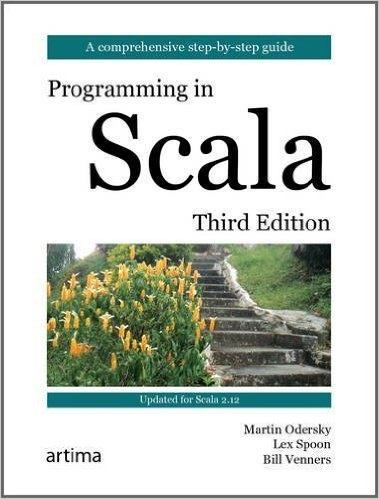
\includegraphics[width=.5\textheight]{white_book}
\caption{The reference guide}
\end{figure}
\end{frame}

\begin{frame}
\begin{figure}
\centering
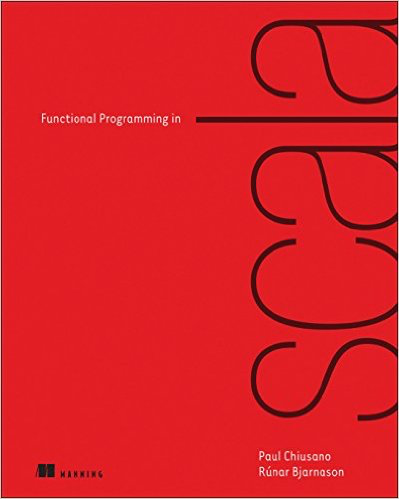
\includegraphics[width=.5\textheight]{red_book}
\caption{Gym to master FP in Scala}
\end{figure}
\end{frame}

\begin{frame}
\begin{figure}
\centering
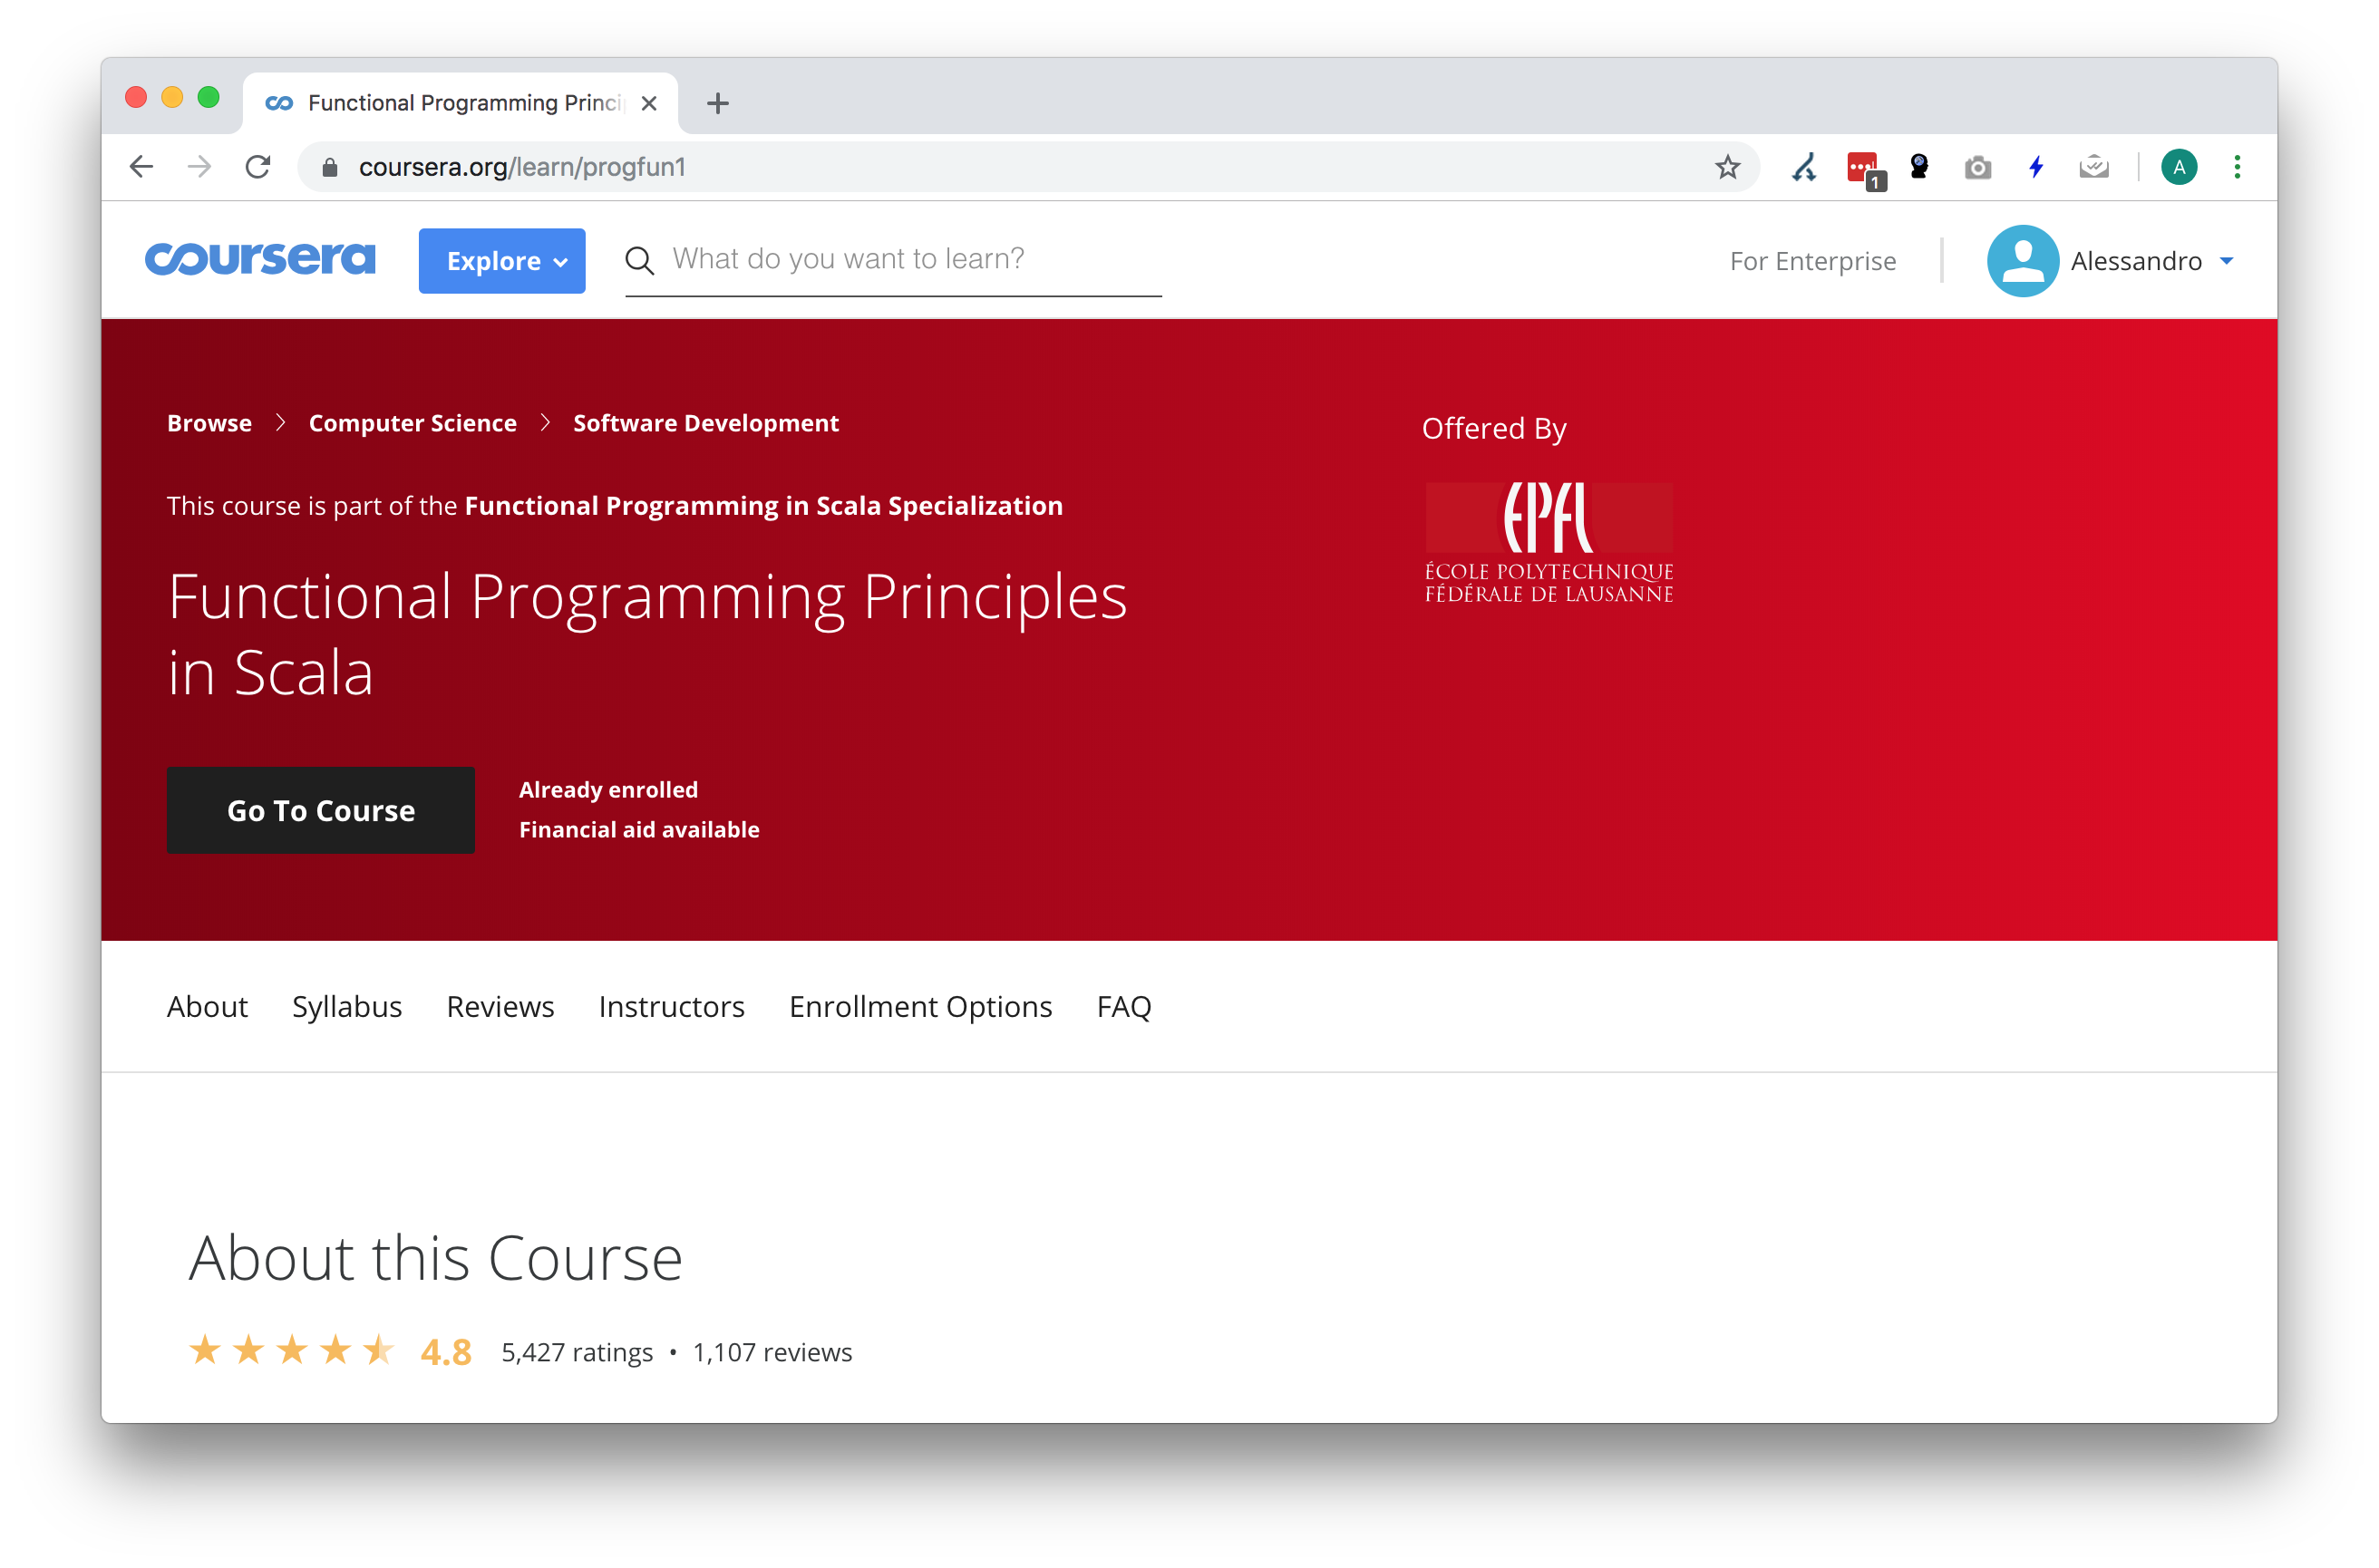
\includegraphics[width=.8\textwidth]{coursera}
\caption{Functional programming principles in Scala MOOC by Martin Odersky}
\end{figure}
\end{frame}

\begin{frame}
Online exercises:
\begin{itemize}
\item \url{https://www.scala-exercises.org/}
\item \url{http://www.scalakoans.org/}
\end{itemize}
\end{frame}

\plain{Questions?}

%\begin{frame}[allowframebreaks] {References}
% \bibliography{demo}
% \bibliographystyle{abbrv}
%\end{frame}

\end{document}
\begin{lstlisting}[language=Kotlin, basicstyle=\ttfamily]
\end{lstlisting}

\begin{frame}
\begin{lstlisting}[language=Kotlin, basicstyle=\ttfamily]
\end{lstlisting}
\end{frame}
